\documentclass[twocolumn]{article}
\usepackage[utf8]{inputenc}
\usepackage[english]{babel}
\usepackage{natbib}
\usepackage{graphicx, caption}
\usepackage{authblk}
\usepackage{textcomp}

% \usepackage{moreverb,savetrees}

\usepackage{multicol}
\usepackage[textwidth=492.982pt, top=2cm, bottom=2cm]{geometry}

\graphicspath{{./figures/}{./}}

\title{Title}
\author[1]{PALAGRAM}

\affil[1]{Affiliations}

\date{}

\newenvironment{Figure}
  {\par\medskip\noindent\minipage{\linewidth}}
  {\endminipage\par\medskip}

\begin{document}

\twocolumn[
	\maketitle

	\begin{abstract}
		Particle-laden gravity currents (PLGCs) are driven by a mass difference between a heavy fluid-particle mixture and a lighter ambient liquid. We focus our attention on finite volume current, generated here by lock-release device over a controlled constant slope bottom at the laboratory scale. The main objective of the present chapter is to provide a comprehensive flow regime associated with the relevant dimensionless parameters which characterize the current at the macroscopic scale, i.e. average over the current depth.
	\end{abstract}
	\vskip 0.7cm
]


%%%%%%%%%%%%%%%%%%%%%%%%%%%%%%%%%%%%%%%%% Figure 1
\begin{figure*}[h]
	\centering
	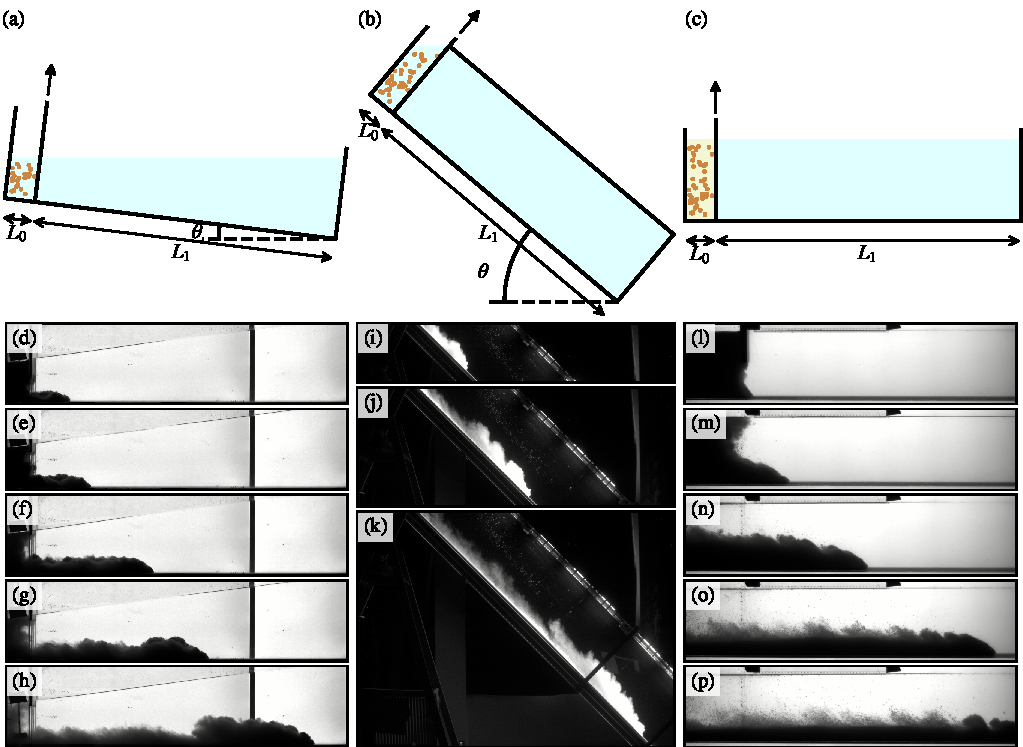
\includegraphics{figure1.pdf}
	\caption{\textbf{Experimental set-ups used in this study.} (a--c) Sketches of the three experimental set-ups. Below are shown snapshots of corresponding experimental images. (d--h) Set-up 1, $\alpha = 7^\circ$, $\phi \sim 3~\%$, $\mathcal{S}t=$ (i--k) Set-up 2, $\alpha = $, $\phi \sim $, $\mathcal{S}t=$ (l--p) Set-up 3, $\alpha = $, $\phi \sim $, $\mathcal{S}t=$.}
	\label{fig:fig1}
\end{figure*}

\section{Introduction}

\subsection{Control parameters}

Particle-laden gravity currents (PLGCs) are driven by a mass difference between a heavy fluid-particle mixture and a lighter ambient liquid. A major difference between compositional currents and PLGCs is therefore the existence of typical length and time scales associated with the particle dynamics. Particularly, the own settling velocity of a heavy particle only allows the existence of these gravity currents on finite time and length scales. Nevertheless, prediction of these finite scales is difficult as it shall strongly depends on the interaction between particle dynamics and the local turbulence of the carrying fluid and/or ambient fluid at the upper interface, which modifies entrainment and associated dissipation, and in turn can delay or enhance settling. Accordingly, their dynamics are controlled by several dimensionless parameters leading to a wide variety of flow regimes. In particular, beyond the slope $\alpha$, the dimensionless density difference between the current and the ambient $At$ and the ratio between available inertia and dissipation, say a Reynolds number $Re$, as usually introduced as a control parameter for compositional currents, the initial solid fraction of particles $\phi$ and a dimensionless settling velocity St have now to be considered as potentially affecting flow regimes. It shall be noted that in some specific situations, some of these dimensionless parameters could be linked as, for instance, $\phi$ and $At$ for heavy particles in a single-phase liquid for the carrying and ambient fluids

\subsection{Literature}


\begin{itemize}
	\item literature slope
	\item literature settling
	\item literature volume fraction
	\item other effects: lock geometry, non-boussinesq, entrainment, erosion/deposition $\rightarrow$ ignored here
\end{itemize}

\section*{Methods}

%%%%%%%%%%%%%%%%%%%%%%%%%%%%%%%%%%%%%%%%%%% Figure 2
\begin{figure}
	\centering
	% \includegraphics{Figures/Figure_lit_plat/Figure_lit_plat.pdf}
	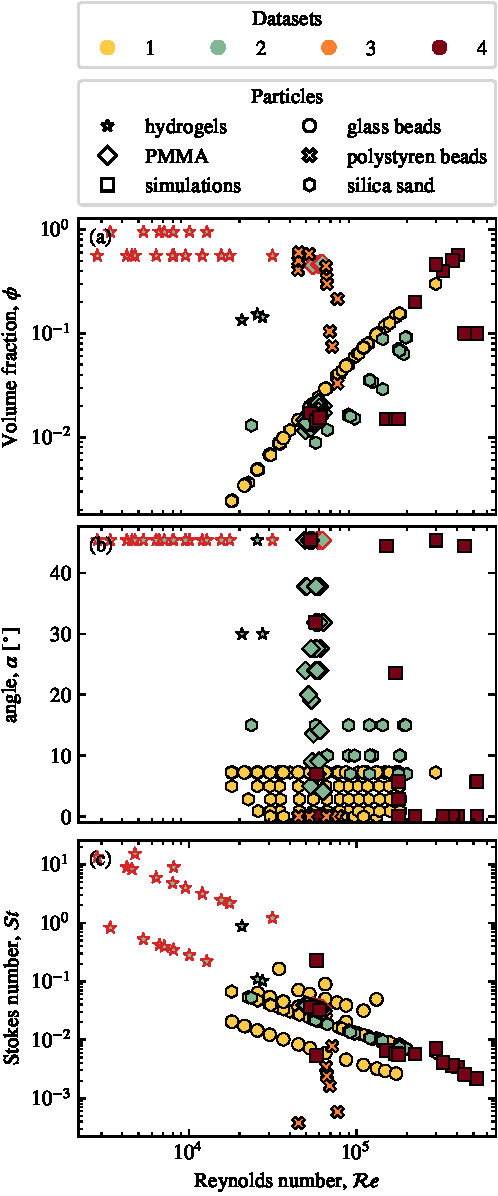
\includegraphics{figure2.pdf}
	\caption{\textbf{Explored parameter space.} Each symbol correspond to a single experimental run.}
	\label{fig:fig2}
\end{figure}


\subsection{Experimental setups}

Even if the dynamics of PLGCs is associated with several complex processes, a general consequence is observed on the front dynamics, often referred to as the $\mathcal{F}r$ number, and the front shape. Then prediction of the different flow regimes associated with PLGCs shall be entirely included into these observables. In order to characterize the different flow regimes for PLGCs induced by a finite volume of material initially at “rest”, 3 dam-break-type devices have been used to cover a wide range of control parameters, as $\alpha \in [0^o,30^o]$, $\phi\in[0.1\%,20\%]$, $At\in[???]$, $Re\in[???]$, $St\in[???]$, $a\in??$, as specifically defined in section \ref{sec:dimensionlessmap}. These experimental devices are supplemented with Euler-Euler numerical simulations to confirm the relevance of such flow regime description to characterize the dynamics of PLGCs.

\subsection{Datasets}

On these 3 devices, a total of $N$ experiments are presented here, complemented by $N$ numerical simulations using SedFoam (see description below). They are classified into 4 different datasets, described below.

\paragraph{Dataset 1}

Description Dataset LEGI

\paragraph{Dataset 2}

Description Dataset IMFT

\paragraph{Dataset 3}

Description Dataset LEGI/IMFT

\paragraph{Dataset 4}

Description Dataset LEMTA

\paragraph{SedFoam}

Description Dataset SedFoam

\subsection{Fitting procedure and front position analysis}

For each experiment/simulation, we extract the current front position as a function of time (see Fig. \ref{fig:fig3}).



%%%%%%%%%%%%%%%%%%%%%%%%%%%%%%%%%%%%%%%%%%%% Figure 3
\begin{figure*}
	\centering
	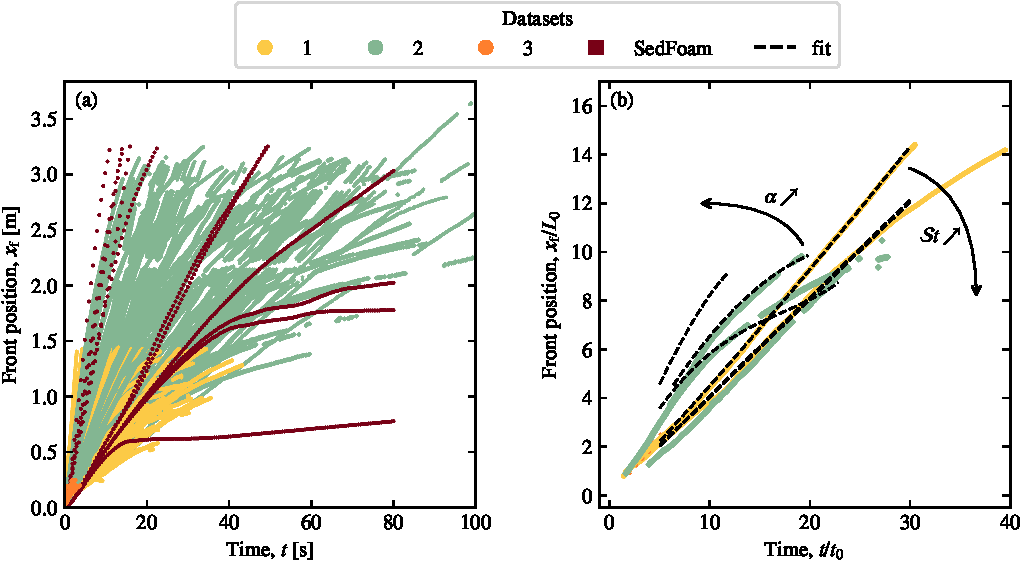
\includegraphics{figure3.pdf}
	\caption{(a) Current front position as a function of time for all experimental runs (b) Selected runs plotted in non-dimensional coordinates.}
	\label{fig:fig3}
\end{figure*}

\section{Dimensional analysis at the macroscopic scale of the current}
\label{sec:dimensionlessmap}

Here, the dimensionless parameters are based on a characteristic length $L_0$ and a characteristic velocity $U_0=\sqrt{g' H_0}$ where $L_0$ and $H_0$ are the horizontal length and depth of the initial container, respectively, $g'$ is the modified gravity $r g \cos{\alpha}$ and $r = (\rho_m - \rho_a)/\rho_a$ with $\rho_m$ and $\rho_a$ the current density and ambient fluid density respectively. Note that $\rho_m = \phi \rho_p+(1-\phi)\rho_f$ with $\rho_p$ the particles density and $\rho_f$ the fluid phase density initially in the current. In the set of experiments presented here $\rho_f\le \rho_a$. The velocity scale $U_0$ corresponds to an idealized transfer of initial potential energy to kinetic energy along the slope, i.e. a collapse of the initial column.


Accordingly,
\begin{equation}
	\displaystyle a =\frac{H_0}{L_0},
\end{equation}
\begin{equation}
	\displaystyle Re = \frac{U_0 H_0\rho_m}{\eta_f},
\end{equation}
\begin{equation}
	\displaystyle At = \frac{\rho_m-\rho_a}{\rho_a},
\end{equation}
\begin{equation}
	\displaystyle St = \frac{V_s}{U_0},
\end{equation}
with $\eta_f$ the interstitial fluid viscosity and $V_s$ the Stokes settling velocity in the interstitial fluid phase labelled $f$.


Then, the dynamics of the current are characterized by several dimensionless variables. The most common one to be analyzed in gravity-driven avalanches is the dimensionless front velocity, also referred to as the Froude number,
\begin{equation}
	\displaystyle \mathcal{F}r =\frac{U_c}{U_0},
\end{equation}
where $U_c$ is the front velocity of the current. Note that $U_c$ is time-dependent, and so is $\mathcal{F}r$, i.e. that $\mathcal{F}r$ as defined here is not a control parameter. (The Froude number which would be defined as a control parameter for a lock-release configuration would be $Fr\equiv 1$, and is thus not relevant to predict the flow dynamics.)

\section{Results}

\subsection{Influence of the slope on the front velocity}

The influence of the slope angle $\alpha$ on the dimensionless front velocity $\mathcal{F}r$ is presented in figure \ref{fig:fig4}. Even if the entire set of experiments and numerical simulations are reported here, results are highlighted for a nearly constant $St\approx 5\times 10^{-2}$ and $\phi < 0.4$ for clarity.

\begin{figure*}
	\centering
	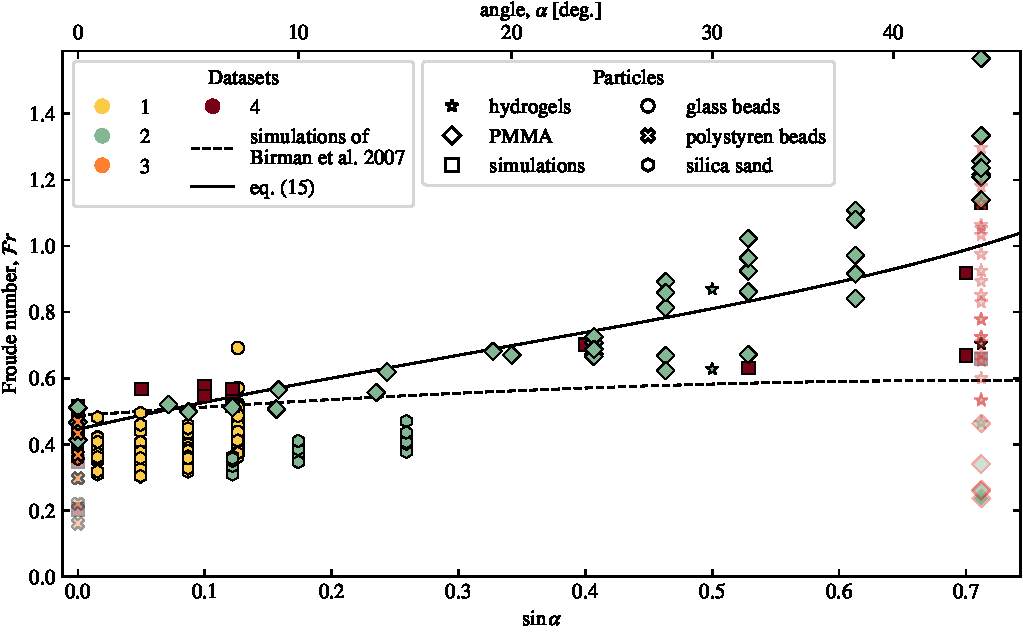
\includegraphics{figure4.pdf}
	\caption{\textbf{Influence of the bottom slope.} (a) Current Froude number as a function of the bottom slope. (b) Current Froude number corrected by a prefector $\sqrt{a}$ as a function of the bottom slope. Here, plain symbols corresponds to $\phi < 0.45$, while transparent symbols are for $\phi \geq 0.45$ (see section~\ref{sec:influence_phi} for details on the influence of $\phi$).}
	\label{fig:fig4}
\end{figure*}

\subsection{Influence of $St$}

\begin{figure*}
	\centering
	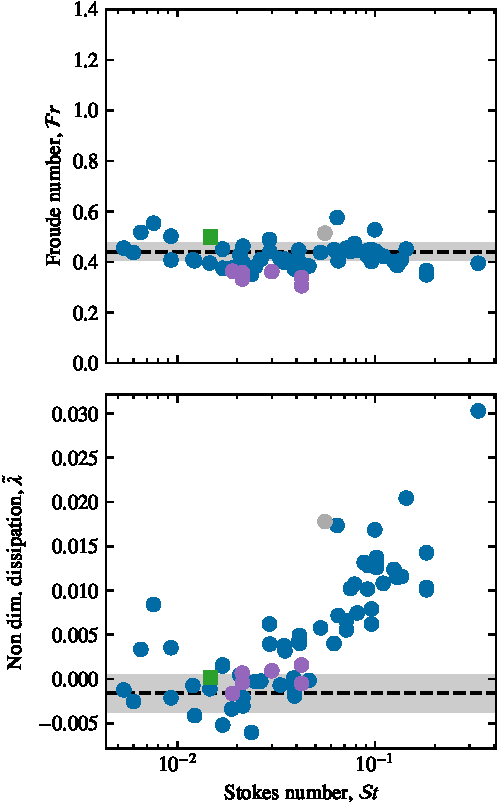
\includegraphics{figure5.pdf}
	\caption{\textbf{Influence of particle settling.} Current Froude number $\mathcal{F}r$ and non-dimensional quadratic dissipation $\tilde{\lambda}$ as a function of the ratio between the Stokes number and the lock aspect-ratio, for different ranges of bottom slopes. Here, we selected runs for $\phi < 0.45$ (see section~\ref{sec:influence_phi} for details on the influence of $\phi$).}
	\label{fig:fig5}
\end{figure*}

Discuss figure \ref{fig:fig5}

\subsection{Influence of volume fraction, $\phi$}
\label{sec:influence_phi}

\begin{figure}
	\centering
	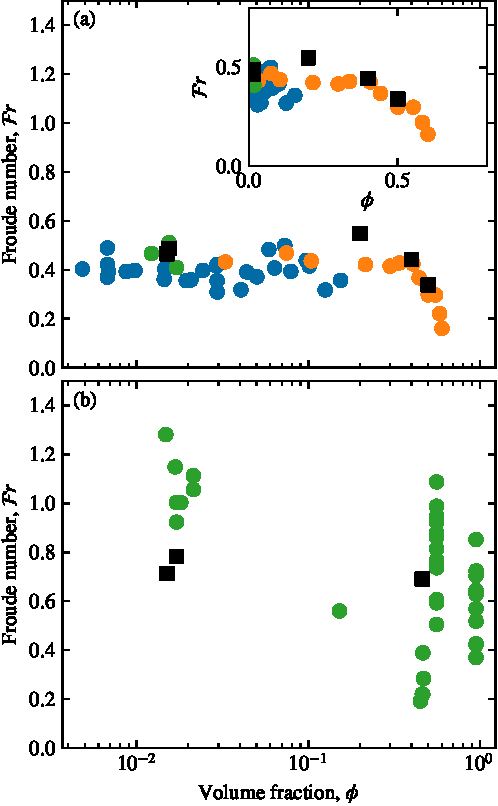
\includegraphics{figure6.pdf}
	\caption{\textbf{Influence of particle volume fraction.} Current Froude number as a function of the initial particle volume fraction for (a) $\alpha \approx 0^\circ$, and (b) $\alpha \approx 45^\circ$. The inset in (a) shows the plot in linear scale.}
	\label{fig:fig6}
\end{figure}

Discuss figure \ref{fig:fig6}


\subsection*{Acknowledgment}

\subsection*{Fundings}


\bibliographystyle{apalike}
\bibliography{biblio}

% \end{multicols*}

\newpage
%TC:endignore

\end{document}
